\chapter{Proposed Methods}

In order to apply some of the previously mentioned topics from the explainability literature to the domain generalization task,  we specifically investigate the usage of gradient class activation maps from \Cref{sec:CAMs}, as well as prototypes from \Cref{sec:prototypes}. Our methods which are based upon these approaches are respectively described in \Cref{sec:divcam} (\divcam), \Cref{sec:prototype_networks} (\prodrop), and \Cref{sec:dtransformers} (\dtransformers).

\section{Diversified Class Activation Maps (\divcam)}
\label{sec:divcam}

\begin{figure}[t]
    \centering
    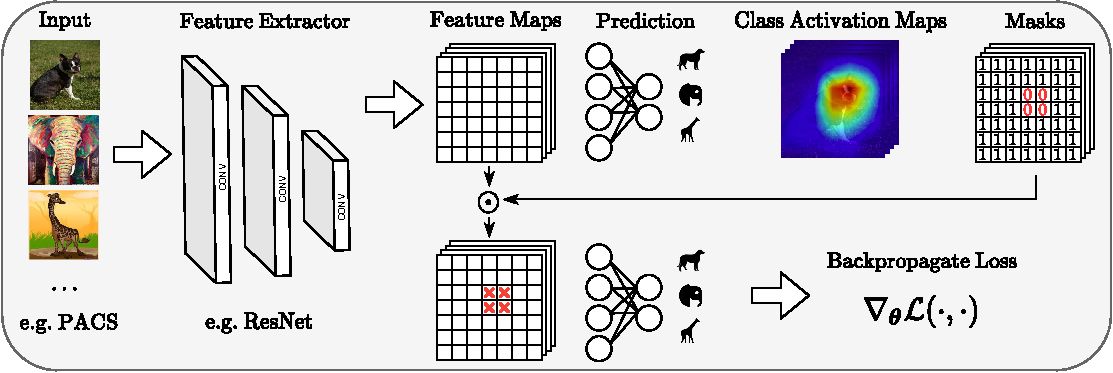
\includegraphics[width=\textwidth]{Figures/Chapter4/model_figure-cropped.pdf}
    \caption{Visualization of the \divcam training process}
    \label{fig:divcam-overview}
\end{figure}


In \Cref{sec:RSC} we introduce the concept of Representation Self-Challenging for domain generalization while in \Cref{sec:CAMs} class activation maps, and specifically Grad-CAM gets introduced. It is quite easy to see that the importance scores $ \Tilde{\mathbf{g}}_{\mathbf{z},c}^k$ in Grad-CAM from \Cref{eq:grad_cam_importance} are a generalization of the spatial mean $\featurega$ used in Channel-Wise RSC from \Cref{eq:ChannelRSCavg}. The spatial mean $\featurega$ only computes the gradient with respect to the features for the most probable class while the importance scores $ \Tilde{\mathbf{g}}_{\mathbf{z},c}^k$ are formulated theoretically for all possible classes but similarly compute the gradient with respect to the feature representation. Both perform spatial average pooling.  

Despite the effectiveness of the model, we believe the approach of \citet{huang2020selfchallenging} does not fully exploit the relation between a feature vector and the actual content of the image. We argue (and experimentally demonstrate) that we can directly use CAMs to construct the self-challenging task. In particular, while the raw target gradient represents the significance of each channel in each spatial location for the prediction, CAMs allow us to better capture the actual importance of each image region. Thus, performing the targeted masking on highest CAM values means explicitly excluding the most relevant \emph{region} of the image that where used for the prediction, forcing the model to focus on other (and interpretable) visual cues for recognizing the object of interests. 

Therefore, as an intuitive baseline, we propose Diversified Class Activation Maps (\divcam), combining the two approaches as shown in \Cref{alg:ActivationMasking} or visualized on a high level in \Cref{fig:divcam-overview}. For that, during each step of the training procedure, we extract the features, compute the gradients with respect to the features as in \Cref{eq:gz}, and perform spatial average pooling to yield $\featurega$ according to \Cref{eq:ChannelRSCavg}. Our method deviates from Channel-Wise RSC by next computing class activation maps $\mathbf{M}_c \in \mathbb{R}^{H_\mathbf{z} \times W_\mathbf{z} \times 1}$ according to \Cref{eq:Map} for the ground truth class label.
\begin{equation}
\label{eq:Map}
    \mathbf{M}_c = \mathtt{max}(0,\sum_{k=1}^K\Tilde{\mathbf{g}}_{\mathbf{z},c}^k \mathbf{z}^k)
\end{equation}
Based on these maps and similar to \Cref{eq:Masking}, we compute a mask $\mathbf{m} \in \mathbb{R}^{H_\mathbf{z} \times W_\mathbf{z} \times 1}$ for the Top-$p$ percentile of map activations as: 
\begin{equation}
\mathbf{m}_{c,i,j}=\left\{\begin{array}{ll}
0, & \text { if } \quad \mathbf{M}_{c, i,j} \geq q_{p} \\
1, & \text { otherwise }
\end{array}\right.
\label{eq:MaskMap}
\end{equation}
As class activation maps and the corresponding masks are averaged along the channel dimension to be specific for each spatial location, we duplicate the mask along all channels to yield a mask with the same size of the features $\mathbf{m} \in \mathbb{R}^{H_\mathbf{z} \times W_\mathbf{z} \times K}$ which can directly be multiplied with the features to mask them and to regularize the training procedure:
\begin{equation}
\label{eq:mutate}
\Tilde{\mathbf{z}} = \mathbf{m} \odot \mathbf{z},
\end{equation}
where $\odot$ is the Hadamard product. The new feature vector $\Tilde{\mathbf{z}}$ is used as input to the classifier $w$ in place of the original $\mathbf{z}$ to regularize the training procedure. For the masked features, we compute the Cross-Entropy Loss from \Cref{eq:cross_entropy} and backpropagate the gradient of the loss to the whole network to update the parameters.

Intuitively, constantly applying this masking for all samples within each batch disregards important features and results in relatively poor performance as the network isn't able to learn discriminative features in the first place. Therefore, applying the mask only for certain samples within each batch as mentioned by \citet[Secton~3.3]{huang2020selfchallenging} should yield a better performance. For convenience, we call this process \emph{mask batching}. On top of that, one could schedule the mask batching with an increasing factor (\eg linear schedule) such that masking gets applied more in the later training epochs where discriminative features have been learned. We apply the mask only if the sample $n$ is within the $(100-b)\mathrm{th}$ percentile of confidences for the correct class (stored in the change vector $\mathbf{c}$ for each sample $n$) and reset the mask otherwise by setting each spatial location $(i,j)$ back to $1$:
\begin{equation}
    \mathbf{m}^n_{c,i,j}=\left\{\begin{array}{ll}
1, & \text { if } \quad \mathbf{c}^n \leq q_{b} \\
-, & \text { otherwise }
\end{array}\right.
\label{eq:MaskingReversion}
\end{equation}
 where $ \mathbf{c}^n$ is is the confidence on the ground truth for sample $n$. This procedure enforces that masks only get applied to samples which are already classified well enough such that the network can now focus on other discriminative properties. For our full ablation study on applying the masks within each batch, please see \Cref{sec:ablation_study_batching}. \Cref{fig:cams_and_masks_divcam} also shows some of the class activation maps produced by \divcam throughout the training procedure.

To try and improve the effectiveness of our CAM-based regularization approach, we can borrow some practices from the weakly-supervised object localization literature. In particular, we explore the use of Homogeneous Negative CAMs (HNC) \citep{sun2020fixing} and Threshold Average Pooling (TAP) \citep{Bae2020RethinkingCAM}. Both methods improve the performance of ordinary CAMs and focus them better on the relevant aspects of an image. See \Cref{sec:abl-masks} for an evaluation of these variants.


\subsection{Global Average Pooling bias for small activation areas}
According to \citet{Bae2020RethinkingCAM}, one problem of traditional class activation maps is that the activated areas for each feature map differ by the respective channels because these capture different class information which isn't properly reflected in the global average pooling operation. Since every channel is globally averaged, smaller feature activation areas result in smaller globally averaged values despite a similar maximum activation value. This doesn't necessarily mean that one of the features is more relevant for the prediction, but can simply be caused by a large area with small activations. To combat this problem, the weight $w_{k,c}$ corresponding to the smaller value, is often trained to be higher when comparing two channels \citep{Bae2020RethinkingCAM}. Instead of the global average pooling operation, they propose \emph{Threshold Average Pooling} (TAP). When adapting their approach for our notation, we receive \Cref{eq:tap} where $\tau_{t a p} = \lambda_{tap} \cdot \mathtt{max}(\Tilde{\mathbf{z}}^k)$ with $\lambda_{tap} \in [0,1)$ as a hyperparameter and $p^k_{tap}$ denotes the scalar from the $k$-th channel of $\mathbf{p}_{tap}$ as it is a $k$-dimensional vector. 
\begin{equation}
\label{eq:tap}
p^k_{tap} =\frac{\sum_{i=1}^{H_\mathbf{z}} \sum_{j=1}^{W_\mathbf{z}} \mathds{1}\left(\Tilde{\mathbf{z}}^k_{i,j} > \tau_{t a p}\right) \Tilde{\mathbf{z}}^k_{i,j}}{\sum_{i=1}^{H_\mathbf{z}} \sum_{j=1}^{W_\mathbf{z}} \mathds{1}\left(\Tilde{\mathbf{z}}^k_{i,j} > \tau_{t a p}\right)}
\end{equation}
When incorporating this into \divcam, this results in changing the global average pooling after self-challenging has been applied to a threshold average pooling. Generally, this plug-in replacement can be seen as a trade-off between \emph{global max pooling} which is better at identifying the important activations of each channel and \emph{global average pooling} which has the advantage that it expands the activation to broader regions, allowing the loss to backpropagate.

\begin{algorithm}[t]
    \SetAlgoLined
    \SetKwInOut{Input}{Input}
    \Input{Data $\mathbf{X}, \mathbf{Y}$ with $\mathbf{x}_i \in \mathbb{R}^{H \times W \times 3}$, drop factor $p,b$, epochs $T$}
    \BlankLine
    \While{$epoch \leq T$}{
        \For{every batch $\mathbf{x}, \mathbf{y}$}{
            Extract features $\mathbf{z} = \phi(\mathbf{x})$ \tcp*[r]{$\mathbf{z}$ has shape  $\mathbb{R}^{H_\mathbf{z} \times W_\mathbf{z} \times K} $}
            Compute $\mathbf{g}_{\mathbf{z},c}$ with \Cref{eq:gz}\;
            Compute $\Tilde{\mathbf{g}}_{\mathbf{z},c}^k$ with \Cref{eq:ChannelRSCavg} \tcp*[r]{$\featurega$ has shape $\mathbb{R}^{1 \times 1 \times K}$}
            Compute $\mathbf{M}_c$ with \Cref{eq:Map} \tcp*[r]{$\mathbf{M}$ has shape $\mathbb{R}^{H_\mathbf{z} \times W_\mathbf{z} \times 1}$}
            Compute $\mathbf{m}_{c,i,j}$ with \Cref{eq:MaskMap} \;
            Repeat mask along channels \tcp*[r]{Afterwards $\mathbf{m}$ has shape $\mathbb{R}^{H_\mathbf{z} \times W_\mathbf{z} \times K}$}
            Adapt $\mathbf{m}_{c,i,j}$ with \Cref{eq:MaskingReversion} \;
            Compute $\Tilde{\mathbf{z}}$ with \Cref{eq:mutate} \;
            Backpropagate loss $\mathcal{L}_{ce}(w(\Tilde{\mathbf{z}}), \mathbf{y})$ \;
            }
    }
\caption{Diversified Class Activation Maps (\divcam)}
\label{alg:ActivationMasking}
\end{algorithm}

\subsection{Smoothing negative Class Activation Maps}
\begin{figure}[t]
    \centering
    \begin{tabularx}{\textwidth}{lYYYY}
       \textbf{Label}  & \textbf{Original} & \textbf{Step 300} & \textbf{Step 2700} & \textbf{Step 4500} \\[0.2cm]
        Giraffe & 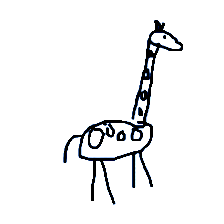
\includegraphics[width=\imagequadsizecams]{Figures/Chapter4/img66.png} &  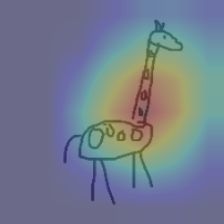
\includegraphics[width=\imagequadsizecams]{Figures/Chapter4/giraffe1_step_300_cam.png} & 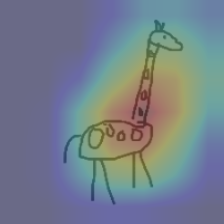
\includegraphics[width=\imagequadsizecams]{Figures/Chapter4/giraffe1_step_2700_cam.png} &
        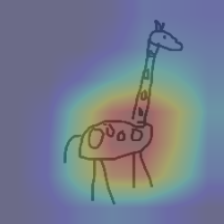
\includegraphics[width=\imagequadsizecams]{Figures/Chapter4/giraffe1_step_4500_cam.png} \\
        Elephant & 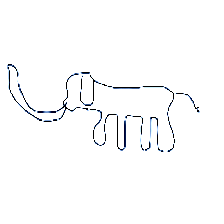
\includegraphics[width=\imagequadsizecams]{Figures/Chapter4/img76.png} &
        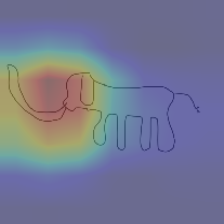
\includegraphics[width=\imagequadsizecams]{Figures/Chapter4/elephant1_step_300_cam.png} &
        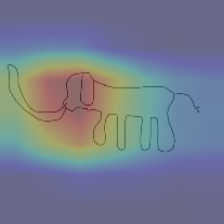
\includegraphics[width=\imagequadsizecams]{Figures/Chapter4/elephant1_step_2700_cam.png} &
        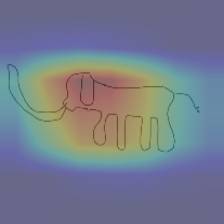
\includegraphics[width=\imagequadsizecams]{Figures/Chapter4/elephant1_step_4500_cam.png} \\
    \end{tabularx}
    \caption[Used class activation maps in \divcams throughout training]{Used class activation maps for \divcams in update step $300/5000$, $2700/5000$, and $4500/5000$ using a ResNet-50 backbone. For the giraffe, we initially focus on the neck while our masks force the network to also take into consideration the overall shape, finally settling on the torso. For the elephant, we initially focus mainly on the elephant trunk and later guide the network towards taking also the shape into consideration.}
    \label{fig:cams_and_masks_divcam}
\end{figure}

Based on the analysis of \citet{sun2020fixing}, negative class activation maps, \ie the class activation maps for classes other than the ground truth, often have false activations even when they are not present in an image. To solve this localization error, they propose a loss function which adds a weighted \emph{homogeneous negative CAM} (HNC) loss term to the existing Cross-Entropy loss. This is shown in \Cref{eq:hnc} where $\lambda_1$ controls the weight of the additional loss term. 
\begin{equation}
\label{eq:hnc}
\mathcal{L}_{neg} =\mathcal{L}_{ce}(\mathbf{y}, w(\Tilde{\mathbf{z}}))+\lambda_1 \mathcal{L}_{hnc}(\mathbf{y}, \boldsymbol{M})
\end{equation}
\citet{sun2020fixing} propose two approaches for implementing $\mathcal{L}_{hnc}$ in their work, both operating on the Top-$m$ most confident negative classes. The first one is based on the mean squared error which suppresses peak responses in the CAMs, while the second one utilizes the Kullback–Leibler (KL) divergence trying to minimize the difference between negative CAMs and an uniform probability map. Since they report similar performance for these variants and the KL loss applies a comparably smoother penalty, we use the KL divergence for our method:
\begin{equation}
\label{eq:hnc-kl}
\mathcal{L}_{hnc}(\mathbf{y}, \boldsymbol{M})=\sum_{c \in J^{m}_>} D_{K L}\left(\boldsymbol{U} \| \boldsymbol{M}_{c}^{\prime}\right).
\end{equation}
Here, $J^{m}_>$ is the set of Top-$m$ negative classes with the highest confidence score, $\boldsymbol{U} \in \mathbb{R}^{H_\mathbf{z} \times W_\mathbf{z}}$ is a uniform probability matrix with all elements having the value $(H_\mathbf{z}W_\mathbf{z})^{-1}$, and $\boldsymbol{M}_{c}^{\prime} = \sigma(\boldsymbol{M}_{c})$ is a probability map produced by applying the softmax function $\sigma$ to each negative class activation map $\boldsymbol{M}_{c}$. Plugging in the definition of the KL divergence and removing the constant as in \Cref{eq:kl-simplification} finally results in a simplified version as
\Cref{eq:hnc-kl-simple}.
\begin{equation}
\label{eq:kl-simplification}
D_{K L}\left(\boldsymbol{U} \| \boldsymbol{M}_{c}^{\prime}\right)=\sum_{i=1}^{H_\mathbf{z}} \sum_{j=1}^{W_\mathbf{z}} \boldsymbol{U}_{i,j} \cdot \log \left( \frac{\boldsymbol{U}_{i,j}}{\boldsymbol{M}_{c, i, j}^{\prime}} \right) =\text { const }-\frac{1}{H_\mathbf{z} W_\mathbf{z}} \sum_{i=1}^{H_\mathbf{z}} \sum_{j=1}^{W_\mathbf{z}} \log \left(\boldsymbol{M}_{c, i, j}^{\prime}\right)
\end{equation}
Generally, with this approach, we add two hyperparametes in the form of the weighting parameter $\lambda$ and the cut-off number $k$ for the Top-$k$ negative classes.
\begin{equation}
\label{eq:hnc-kl-simple}
    \mathcal{L}_{hnc}(\mathbf{y}, \boldsymbol{M})= -\frac{1}{H_\mathbf{z} W_\mathbf{z}} \sum_{c \in J^{m}_>} \sum_{i=1}^{H_\mathbf{z}} \sum_{j=1}^{W_\mathbf{z}} \log \left(\boldsymbol{M}_{c, i, j}^{\prime}\right)
\end{equation}
Since we use Grad-CAMs instead of ordinary CAMs in \divcam, na\"{i}vely applying this would require computing the gradient for every negative class $c$ in the set $J^m_>$ which would result in computing \Cref{eq:hnc-kl-grad-cam} where $y_c$ is the confidence of the negative class. 
\begin{equation}
\label{eq:hnc-kl-grad-cam}
    \mathcal{L}_{hnc}(\mathbf{y}, \boldsymbol{M})= -\frac{1}{H_\mathbf{z} W_\mathbf{z}} \sum_{c \in J^{m}_>} \sum_{i=1}^{H_\mathbf{z}} \sum_{j=1}^{W_\mathbf{z}} \log \left( \sigma \left(\mathtt{max}\left(0,\sum_{k=1}^K\left(\frac{1}{H_\mathbf{z}W_\mathbf{z}} \sum_{i=1}^{H_\mathbf{z}} \sum_{j=1}^{W_\mathbf{z}} \frac{\partial y_c}{\partial \mathbf{z}_{i,j}^k}\right)^k \mathbf{z}^k\right)\right)\right)
\end{equation}
To speed up the training for tasks with a large number of classes, we approximate the loss by summing the negative class confidences before backpropagating as shown in \Cref{eq:hnc-kl-grad-cam-approx}. This amounts to considering all negative classes within $J^\prime_>$ as one negative class. 
\begin{equation}
\label{eq:hnc-kl-grad-cam-approx}
    \widehat{\mathcal{L}}_{hnc}(\mathbf{y}, \boldsymbol{M})= -\frac{1}{H_\mathbf{z} W_\mathbf{z}} \sum_{i=1}^{H_\mathbf{z}} \sum_{j=1}^{W_\mathbf{z}} \log \left( \sigma \left(\mathtt{max}\left(0,\sum_{k=1}^K\left(\frac{1}{H_\mathbf{z}W_\mathbf{z}} \sum_{i=1}^{H_\mathbf{z}} \sum_{j=1}^{W_\mathbf{z}} \frac{\partial \sum_{c \in J^{m}_>} y_c}{\partial \mathbf{z}_{i,j}^k}\right)^k \mathbf{z}^k\right)\right)\right)
\end{equation}
To finally implement this into \divcam, we simply substitute the current loss $\mathcal{L}_{ce}(\mathbf{y}, w(\Tilde{\mathbf{z}}))$ in line $12$ from \Cref{alg:ActivationMasking} with \Cref{eq:hnc} where $\mathcal{L}_{hnc}(\mathbf{y}, \boldsymbol{M})$ is implemented through our approximation $\widehat{\mathcal{L}}_{hnc}(\mathbf{y}, \boldsymbol{M})$ given in \Cref{eq:hnc-kl-grad-cam-approx}. 


Next, we can try to utilize domain information in \divcam by aligning distributions of class activation maps produced by the same class across domains. We want their distributions to align as close as possible such that we cannot identify which domain produced which class activation map. For that, we can utilize some methods previously introduced in \Cref{sec:invariant_features}, in particular we explore minimizing the sample maximum mean discrepancy introduced in \Cref{eq:mmd} and using a conditional domain adversarial neural network (CDANN). See \Cref{sec:abl-masks} for an evaluation of these variants.


\subsection{Conditional Domain Adversarial Neural Networks}
We combine the domain adversarial neural network (CDANN) approach, originally introduced by \citet{LiTGLLZT18}, with \divcam to align the distributions of CAMs across domains. For that, we try to predict the domain to which a class activation map belongs by passing it to a multi-layer perceptron $\omega$. We compute the cross entropy loss between the predictions and the domain ground truth $\mathbf{d}$ and weight it for each sample by the occurrence probability of the respective class.
After weighting, we can sum up all the losses and add it to our overall loss, weighted by $\lambda_2$:
\begin{equation}
\label{eq:adv}
\mathcal{L}_{adv} =\mathcal{L}_{ce}(\mathbf{y}, w(\Tilde{\mathbf{z}}))+\lambda_2 ( \mathcal{L}_{ce}(\mathbf{d}, \omega(\boldsymbol{M})) + \eta \left\|\nabla_{\boldsymbol{M}} \mathcal{L}_{ce}(\mathbf{d}, \omega(\boldsymbol{M}))\right\|_2).
\end{equation}
During each training step, we either update the discriminator, \ie the predictor for the domain, or the generator, \ie the main network including featurizer and classifier. The discriminator loss inherently includes a $\ell^2$ penalty on the gradients, weighted by $\eta$.


\subsection{Maximum Mean Discrepancy}

Given two samples $\mathbf{x}^{\xi_1}$ and $\mathbf{x}^{\xi_2}$ drawn from two individual, unknown  domain distributions $\mathcal{D}_{\xi_1}$ and $\mathcal{D}_{\xi_2}$, the maximum mean discrepancy (MMD) is given by \Cref{eq:mmd_maps} where $\varphi: \mathbb{R}^{d} \rightarrow \mathcal{H}$ is a feature map and $k(\cdot, \cdot)$ is the kernel function induced by $\varphi(\cdot)$. We consider every distinct pair of source domains $(\xi_u, \xi_v)$, representing training domains $\xi_u$ and $\xi_v$, with $\xi_u\neq \xi_v$ to be in the set $\mathfrak{P}$.
\begin{equation}
\label{eq:mmd_maps}
    \mathcal{L}_{dist} =\sum_{\xi_u,\xi_v \in \mathfrak{P}}\left\|\mathbb{E}_{\mathbf{x}^{\xi_u} \sim \mathcal{D}_{\xi_u}}[\varphi(\featureex(\mathbf{x}^{\xi_u}))]-\mathbb{E}_{\mathbf{x}^{\xi_v} \sim \mathcal{D}_{\xi_v}}[\varphi(\featureex(\mathbf{x}^{\xi_v}))]\right\|_{\mathcal{H}}
\end{equation}
In simpler terms, we map features into a reproducing kernel Hilbert space $\mathcal{H}$, and compute their mean differences within the RKHS. This loss pushes samples from different domains, which represent the same class, to lie nearby in the embedding space. According to \citet{SriperumbudurFGLS09}, this mean embedding is injective, \ie arbitrary distributions are uniquely represented in the RKHS, if we use a characteristic kernel. For this work, we choose the gaussian kernel shown in \Cref{eq:gaussian_kernel} which is a well-known characteristic kernel.
\begin{equation}
\label{eq:gaussian_kernel}
    k(x,x') = \exp \left(-\frac{\|x-x'\|^{2}}{2 \sigma^{2}}\right)
\end{equation}
Since the choice of kernel function can have a significant impact on the distance metric, we adopt the approach of \citet{LiPWK18} and use a mixture kernel by averaging over multiple choices of $\sigma$ as already implemented in \domainbed. This gets incorporated into our loss function weighted by $\lambda_3$ with:
\begin{equation}
    \mathcal{L}_{mmd} = \mathcal{L}_{ce}(\mathbf{y}, w(\Tilde{\mathbf{z}}))+\lambda_3 \mathcal{L}_{dist}.
\end{equation}
With this approach, we inherently align the computed masks by aligning the individual samples from different domains, aiming at producing domain invariant masks. This procedure can be applied at different levels \eg on the features, class activation maps, or masked class activation maps. In \Cref{sec:abl-masks}, we only provide results for the feature level due to the effectiveness that similar approaches showed in \domainbed. However, we observe a similar trend for the other application levels as well.

\section{Prototype Networks for Domain Generalization}
\label{sec:prototype_networks}

Another approach to combine explainability methods with the task of domain generalization is to use the prototype method outlined in \Cref{sec:prototypes}.  In particular, we can directly adapt the approach of \citet{ChenLTBRS19} as a baseline where we associate each class with a pre-defined number of prototypes. The cluster and separation losses from \Cref{eq:prototype_losses} ensure that each prototype resembles a prototypical attribute for the associated class and we minimize them according to \Cref{eq:min_prototypes}.

\begin{figure*}[t]
    \centering
    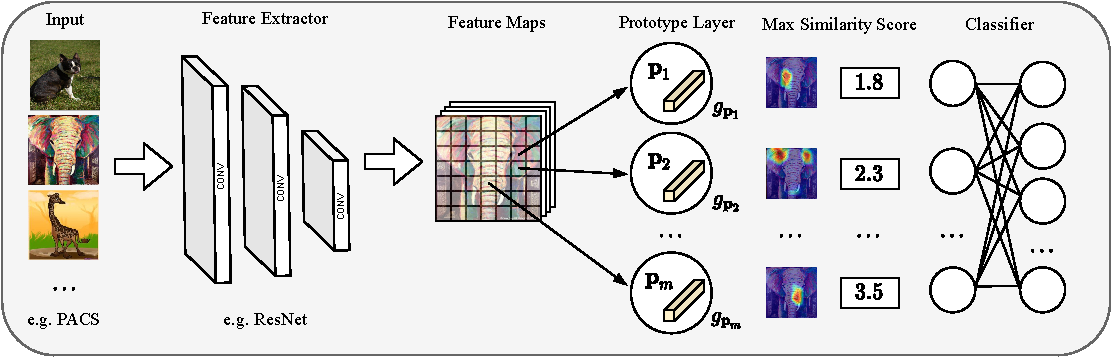
\includegraphics[width=\textwidth]{Figures/Chapter4/prototype_agnostic-cropped.pdf}
    \caption{Domain-agnostic Prototype Network}
    \label{fig:domain_prototype_network}
\end{figure*}

For our application scenario, this prototype layer is used after the domain-agnostic featurizer $\phi$ and operates on the features like illustrated in \Cref{fig:domain_prototype_network}. As each prototype is trained with data from all training domains $\Xi$, they become inherently domain agnostic. This baseline uses a joint classifier $w$ to output the final prediction which operates on the maximum similarity for all the prototypes and \emph{some} latent patch. Similar to \citet{ChenLTBRS19}, we preface the prototype layer with two convolutional layers with kernel size $1$, a ReLU function between them, and finally a sigmoid activation function. We observe that having roughly $100$ initial update steps where only these in-between layers are trained is crucial for competitive performance. We anticipate that these steps are used to adapt the randomly-initialized convolutional weights to the image statics imposed by the pre-trained backbone.\footnote{Further implementation details can be found here: \url{https://github.com/SirRob1997/DomainBed/}} While this baseline is meaningful, we also consider a second variant where we build an ensemble of prototype layers, each learning domain-specific prototypes.


\subsection{Ensemble Prototype Network}
Following the intuition provided by works that utilize model ensembling, which have been described in \Cref{sec:model_ensembling}, we can use domain information by up-scaling the network to use a prototype layer for each domain separately. For the PACS dataset, this would correspond to having three prototype layers, one for each training domain \eg a photo, art, and cartoon prototype layer when predicting sketch images. Each prototype layer is only trained with images from their corresponding domain.

As shown in \Cref{fig:ensemble_prototype_network}, we associate each domain with both a prototype layer and a classifier which takes similarity scores of that domain's prototypes as input. During training, we only feed images of the associated domain to the respective prototype layer and classifier to enforce this domain correspondence. The aggregation weights of the final linear layer are set to a one-hot encoding representing the correct domain. During testing, we can then feed the new unseen domain to each domain prototype layer, allowing each domain's prototypes to influence the final prediction. 

There exist multiple strategies for setting the aggregation weights during this stage. The most simple version is to set the influence of each domain uniform, \ie if we have three training domains the connections from each domain would have the weight $\frac{1}{3}$ such that each domain has the same influence on the final prediction. Our second approach is to jointly train a domain predictor to output the weights for the aggregation layer which can either be used both, during training and testing, or only during testing, similar to what is done by \citet{ManciniBC018}. This method allows for a more flexible aggregation of the separated predictions coming from the different prototype layers, enabling the network to put more emphasis on the relevant domain prototypes.  

\begin{figure*}[t]
    \centering
    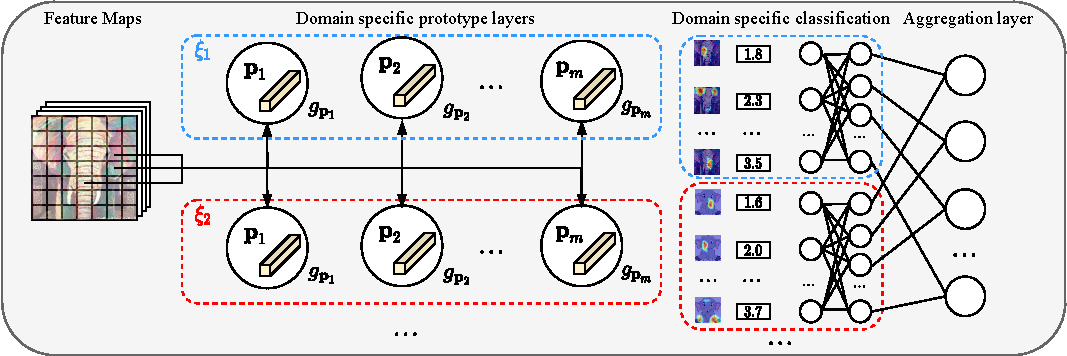
\includegraphics[width=\textwidth]{Figures/Chapter4/prototype_ensemble-cropped.pdf}
    \caption{Ensemble Prototype Network}
    \label{fig:ensemble_prototype_network}
\end{figure*}

Lastly, we also experiment with an ensemble variant that is specific to prototype layers. Instead of only pre-defining a number of prototypes for each class in the domain agnostic prototype layer outlined in \Cref{sec:prototype_networks}, we can also pre-define domain correspondence for each prototype. Training is then done by passing each domain separately to the prototype layer and masking the overall prototype outputs if they do not correspond to the current environment. The cluster and separation losses are adapted to an average over the individual environments as:
\begin{alignat}{3}
\label{eq:prototype_losses_domain}
    \mathcal{L}_{\mathrm{clst}} &= \frac{1}{s} \sum_{\env \in \envs} &&\frac{1}{n_\env} \sum_{i=1}^{n_\env} \min_{j: \prot\in \prots_{\yyi}^\env} \min_{\zpatch \in \text{patches}(\zz^\env)} \left\|\zpatch - \prot\right\|^2_2\\
    \mathcal{L}_{\mathrm{sep}} &= \frac{1}{s} \sum_{\env \in \envs}-&&\frac{1}{n_\env} \sum_{i=1}^{n_\env} \min_{j: \prot \notin \prots_{\yyi}^\env} \min_{\zpatch \in \text{patches}(\zz^\env)} \left\|\zpatch - \prot\right\|^2_2,
\end{alignat}
where $\prots_{\yyi}^\env$ denotes the prototypes associated with the specific class \emph{and} environment while $\zz^\env$ denotes the latent representation of an image corresponding to the current domain. This ensemble variant inherently removes the need for setting appropriate aggregations weights as prototype activations are simply masked during training while during testing all prototypes are kept, allowing each prototype from each source domain to influence the prediction.  With a domain specific cross entropy loss:
\begin{equation}
    \lterm_{\mathrm{ce}} = \frac{1}{s} \sum_{\env \in \envs} \frac{1}{n_\env} \sum_{i=1}^{n_\env} -\sum_{c=1}^{C} y_{i, c}^{\env} \cdot \log \left(\hat{y}_{i, c}^{\env}\right),
\end{equation}
we optimize the final loss of our ensemble model as:
\begin{equation}
    \lterm = \lterm_{\mathrm{ce}} + \lambda_{\mathrm{clst}} \mathcal{L}_{\mathrm{clst}} + \lambda_{\mathrm{sep}} \mathcal{L}_{\mathrm{sep}}.
\end{equation}
While all of these ensemble variants \emph{should} work given the intuition from previous works that have been using model ensembles for learned domain-specific latent spaces, we observe that these assumptions do \emph{not} hold for prototype networks based on our additional experiments of the proposed variants. For us, any prototype ensemble was consistently outperformed by one domain-agnostic prototype layer. 

\subsection{Diversified Prototypes (\prodrop)}
\label{sec:divpro}

Initial experiments with both domain-agnostic and domain-specific prototype layers lead to unsatisfactory results. To investigate this behavior, we analyze the pairwise prototype $\ell_2$-distance as well as the cosine-distance $\cdistance$ which for any two prototypes $\proti_i$ and $\prot$ are given by:
\begin{alignat}{3}
\label{eq:pairwise_prot_distances}
    &\ell_2 &&= &&\left\|\proti_i - \prot  \right\|_2\\ 
    &\cdistance &&= 1- &&\frac{\proti_i\prot}{\left\|\proti_i \right\|_2 \left\|\prot \right\|_2} .
\end{alignat}
Through the $\ell_2$-distance we can grasp the euclidean distance between any two prototypes while the cosine-distance $\cdistance \in [0,2]$ is the inverted version of the cosine similarity which is a metric to judge the cosine of the angle between them. Here, we visualize the cosine-distance instead of the cosine similarity to match the color-scheme of the $\ell_2$-distance \ie low values resemble closeness. 

The results of this analysis can be seen in \Cref{fig:pw_distance_trial1} and \Cref{fig:pw_distance_trial1-sc} for the first data split and a negative weight of $w_{c,j} = -1.0\; \forall j: \prot \notin \prots_c$ but we also show the same plots for $w_{c,j} = 0.0$ and the two additional data splits in \Cref{sec:additional_distances}. As both of the used metrics are symmetric, only the upper triangle is visualized. We observe that depending on the data split and negative weight, the model sometimes converges to having one or two prototypes per class that have a large $\ell_2$ distance while many of the other prototypes are close. Striking examples for this behavior can be seen in \Cref{fig:pairwise_distance} for the sketch domain or in \Cref{fig:pw_distance_trial1} for the sketch and cartoon domain. This observation suggests, that in these scenarios the model fails to properly use all of the available prototypes and only relies on a significantly reduced subset per class, not training the other prototypes. In relation to the cosine-distance, however, we can often observe that exactly these prototypes with a high pairwise $\ell_2$-distance to all the other prototypes have a slightly lower cosine-distance. Such behavior can be seen for example in \Cref{fig:pairwise_distance} in the art and cartoon environment or in \Cref{fig:pw_distance_trial1} for the sketch and cartoon domain. For the most part, many cosine-distances tend to be low and more or less uniformly spaced. Nevertheless, we can occasionally identify ``streaking'' patterns in the cosine-distances where prototypes for certain classes are well-spaced but they have a larger (or equal) cosine-distance to prototypes of other classes. See for example \Cref{fig:pairwise_distance} for the sketch domain, \Cref{fig:pw_distance_0.0_trial1} for the sketch and photo domain, and \Cref{fig:pw_distance_0.0_trial2}  for the sketch and cartoon domain.

\begin{figure}[t]
    \centering
    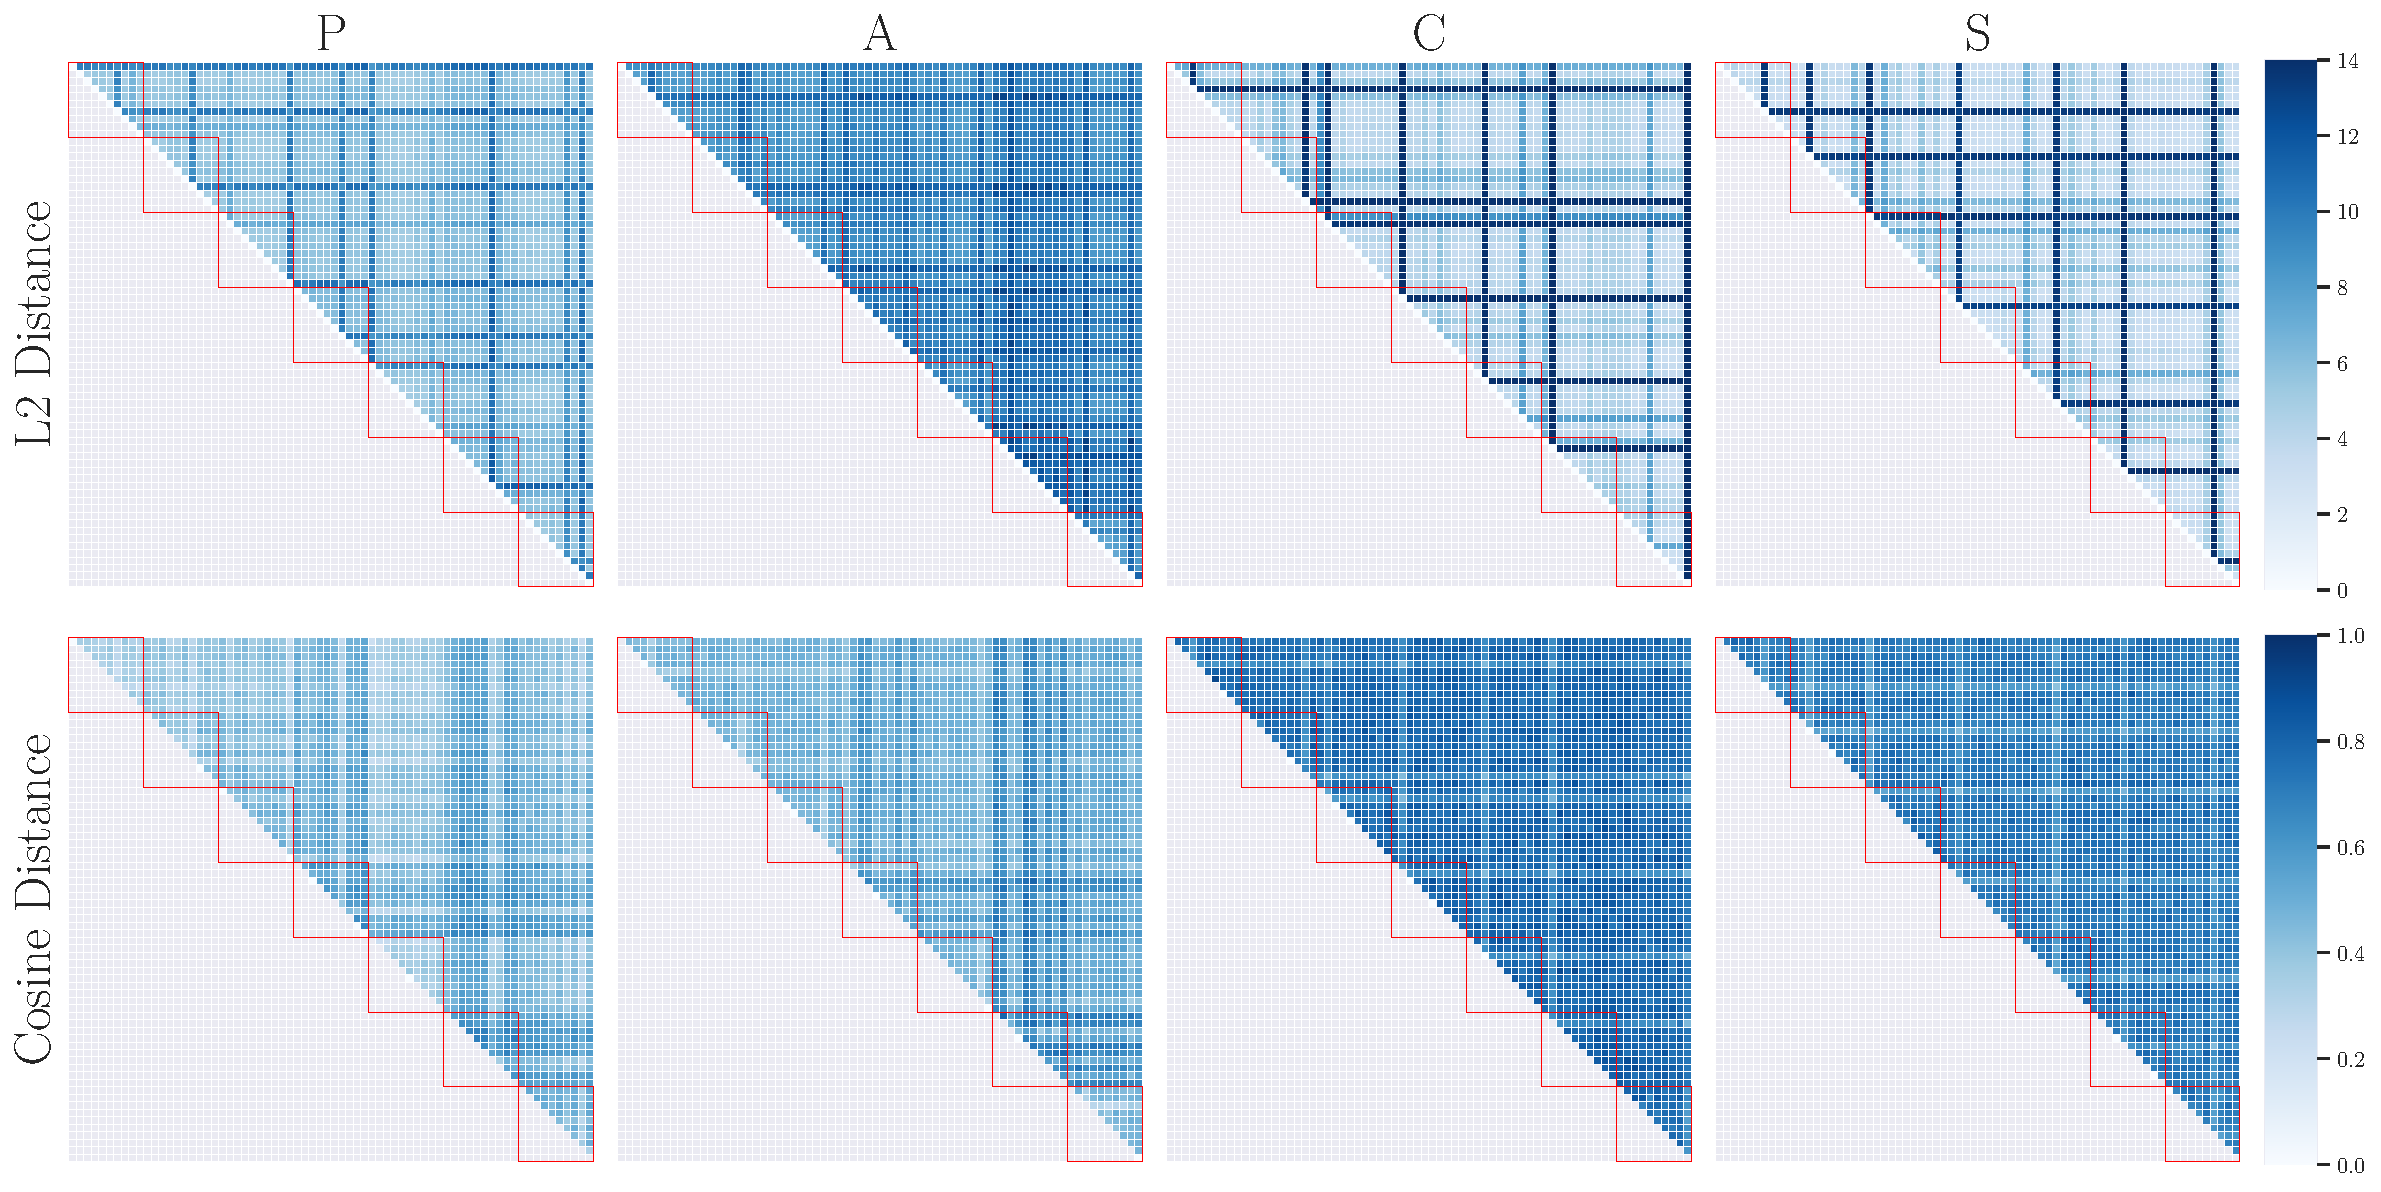
\includegraphics[width=\textwidth]{Figures/Chapter4/2021-01-21-ProDropIncorrectWeight-1.0SAVEResNet18oracle_validation_trial1.pdf}
    \caption[Second data split pairwise prototype distances with $w_{c,j} = -1.0$] {Pairwise learned prototype $\ell_2$-distance (top) and cosine-distance $\cdistance$ (bottom) of the best-performing model with negative weight $w_{c,j} = -1.0\; \forall j: \prot \notin \prots_c$ for each testing domain. Red squares denote prototype class correspondence for the $7$ different classes in the PACS dataset. No self-challenging is applied and colormap bounds are adjusted per metric for visualization purposes. Second data split.}
    \label{fig:pw_distance_trial1}
\end{figure}

From a design standpoint, we would like the prototypes within each class to be reasonably well spaced out in the latent space such that they can resemble different discriminative attributes about each class. That is, we would like the network to utilize all the prototypes and not only rely on a small subset of prototypes or discriminative features for their prediction. The distances of these prototypes to the prototypes of the other classes, however, should \emph{not} be restrained in any way and should be learned automatically. For example, when predicting different bird species, this allows the network to place similar head prototypes of different classes closer together. The existing cluster and separation losses enforce that each prototype associated with that class is close to at least one latent patch of that class while maximizing the distance to the prototypes of other classes. However, this does not enforce that each prototype associated with that class acts on a different discriminative feature.

One approach to possibly enforce this behavior is to incorporate the self-challenging method previously applied to \divcam to the presented prototype network resulting in a novel algorithm we call \emph{prototype dropping} (\prodrop) which is described in \Cref{alg:ProDrop}. In essence, we extract features by passing our input images to the featurizer $\mathbf{z} = \phi(\mathbf{x})$ and compute the similarity scores for each prototype by passing it to the prototype layer $\unit(\zz)$ with \Cref{eq:prot_layer_function}. Based on these similarity scores, we compute a mask $\mathbf{m}_{c,j}$ for the prototypes of the respective class $c$ with the Top-$p$ highest activation:
\begin{equation}
\mathbf{m}_{c,j}=\left\{\begin{array}{ll}
0, & \text { if } \quad \unit(\zz) \geq q_{c, p}\quad \forall j: \prot \in \prots_c \\
1, & \text { otherwise },
\end{array}\right.
\label{eq:ProDropFeatureMask}
\end{equation}
where $q_{c, p}$ is the corresponding threshold value. We also apply the mask batching from \divcam without scheduling which only applies this type of masking for the highest confidence samples on the ground truth. Finally, we can mask the samples using the Hadamard product $\odot$ with:
\begin{equation}
\label{eq:mutate_prodrop}
\mplayer(\zz) = \mathbf{m} \odot \player(\zz).
\end{equation}
In practice, all of these operations can be efficiently implemented using \texttt{torch.quantile}, \texttt{torch.lt}, and \texttt{torch.logical\_or} on small tensors, all of which pose no significant computational overhead.

\begin{algorithm}[t]
    \SetAlgoLined
    \SetKwInOut{Input}{Input}
    \Input{Data $\mathbf{X}, \mathbf{Y}$ with $\mathbf{x}_i \in \mathbb{R}^{H \times W \times 3}$, drop factor $p,b$, epochs $T$}
    \BlankLine
    \While{$epoch \leq T$}{
        \For{every batch $\mathbf{x}, \mathbf{y}$}{
            Extract features $\mathbf{z} = \phi(\mathbf{x})$ \tcp*[r]{$\mathbf{z}$ has shape  $\mathbb{R}^{H_\mathbf{z} \times W_\mathbf{z} \times K} $}
            Compute $\unit(\zz)$ with \Cref{eq:prot_layer_function}\;
            Compute $\mathbf{m}_{c,j}$ with \Cref{eq:ProDropFeatureMask} \;
            Adapt $\mathbf{m}_{c,j}$ with \Cref{eq:MaskingReversion} \;
            Compute $\mplayer(\zz)$ with \Cref{eq:mutate_prodrop} \;
            Backpropagate loss $\mathcal{L}_{ce}(w(\mplayer(\zz)), \mathbf{y}) + \lambda_4 \mathcal{L}_{\mathrm{clst}} + \lambda_5 \mathcal{L}_{\mathrm{sep}}$ \;
            }
    }
\caption{Prototype Dropping (\prodrop)}
\label{alg:ProDrop}
\end{algorithm}


The effect of this approach on the pairwise prototype distances can be seen in \Cref{fig:pairwise_distance_sc} as well as \Cref{sec:additional_distances}. We observe, that even though self-challenging helps to boost the overall performance (see \Cref{sec:abl_self_challenging}), it does not particularly well achieve the previously described desired distance properties and only improves them marginally. Positive effects can be seen in \Cref{fig:pw_distance_trial1-sc} for the sketch and cartoon domain, \Cref{fig:pw_distance_0.0_trial2-sc} for the sketch domain, or \Cref{fig:pw_distance_0.0_trial1-sc} for the cartoon domain.

Our second approach to enforce the desired distance structures is to add an additional intra-class prototype loss term $\mathcal{L}_\mathrm{intra}$ which maximizes the intra-class prototoype $\ell_2$- and/or cosine-distance weighted by $\lambda_6$. Again, this loss term can \emph{in theory} have a few different definitions depending on the chosen distance metrics, we experiment with: 
\begin{equation}
\label{eq:intra_loss}
    \mathcal{L}_\mathrm{intra} = \sum_{\proti_i, \prot \in \prots_c} \lambda_{\ell_2} \underbrace{\left\|\proti_i - \prot  \right\|_2 \vphantom{\frac{\proti_i\prot}{\left\|\proti_i \right\|_2 \left\|\prot \right\|_2}}}_{\ell_2-\text{distance}} + \lambda_{\cdistance} \underbrace{ (1-\frac{\proti_i\prot}{\left\|\proti_i \right\|_2 \left\|\prot \right\|_2})}_{\text{cosine-distance}},
\end{equation}
where the $\ell_2$-distance and the cosine-distance are weighted by $\lambda_{\ell_2}$ and $\lambda_{\cdistance}$ respectively. Performance results for the loss presented in \Cref{eq:intra_loss} with $\lambda_{\ell_2} = 1$ and $\lambda_{\cdistance} = 1$ are shown in \Cref{sec:intra_loss}. Since the cosine-distance is bounded, this commonly amounts to the $\ell_2$-distance having a higher influence. We also experimented with other values for $\lambda_{\ell_2}$ and $\lambda_{\cdistance}$, such as setting either one of them to zero and only applying either the $\ell_2$- or the cosine-distance ($\lambda_{\ell_2} = 0$, $\lambda_{\cdistance} = 1$ and $\lambda_{\ell_2} = 1$, $\lambda_{\cdistance} = 0$), but couldn't find any further benefits by canceling or re-weighting them differently. 

\begin{figure}[t]
    \centering
    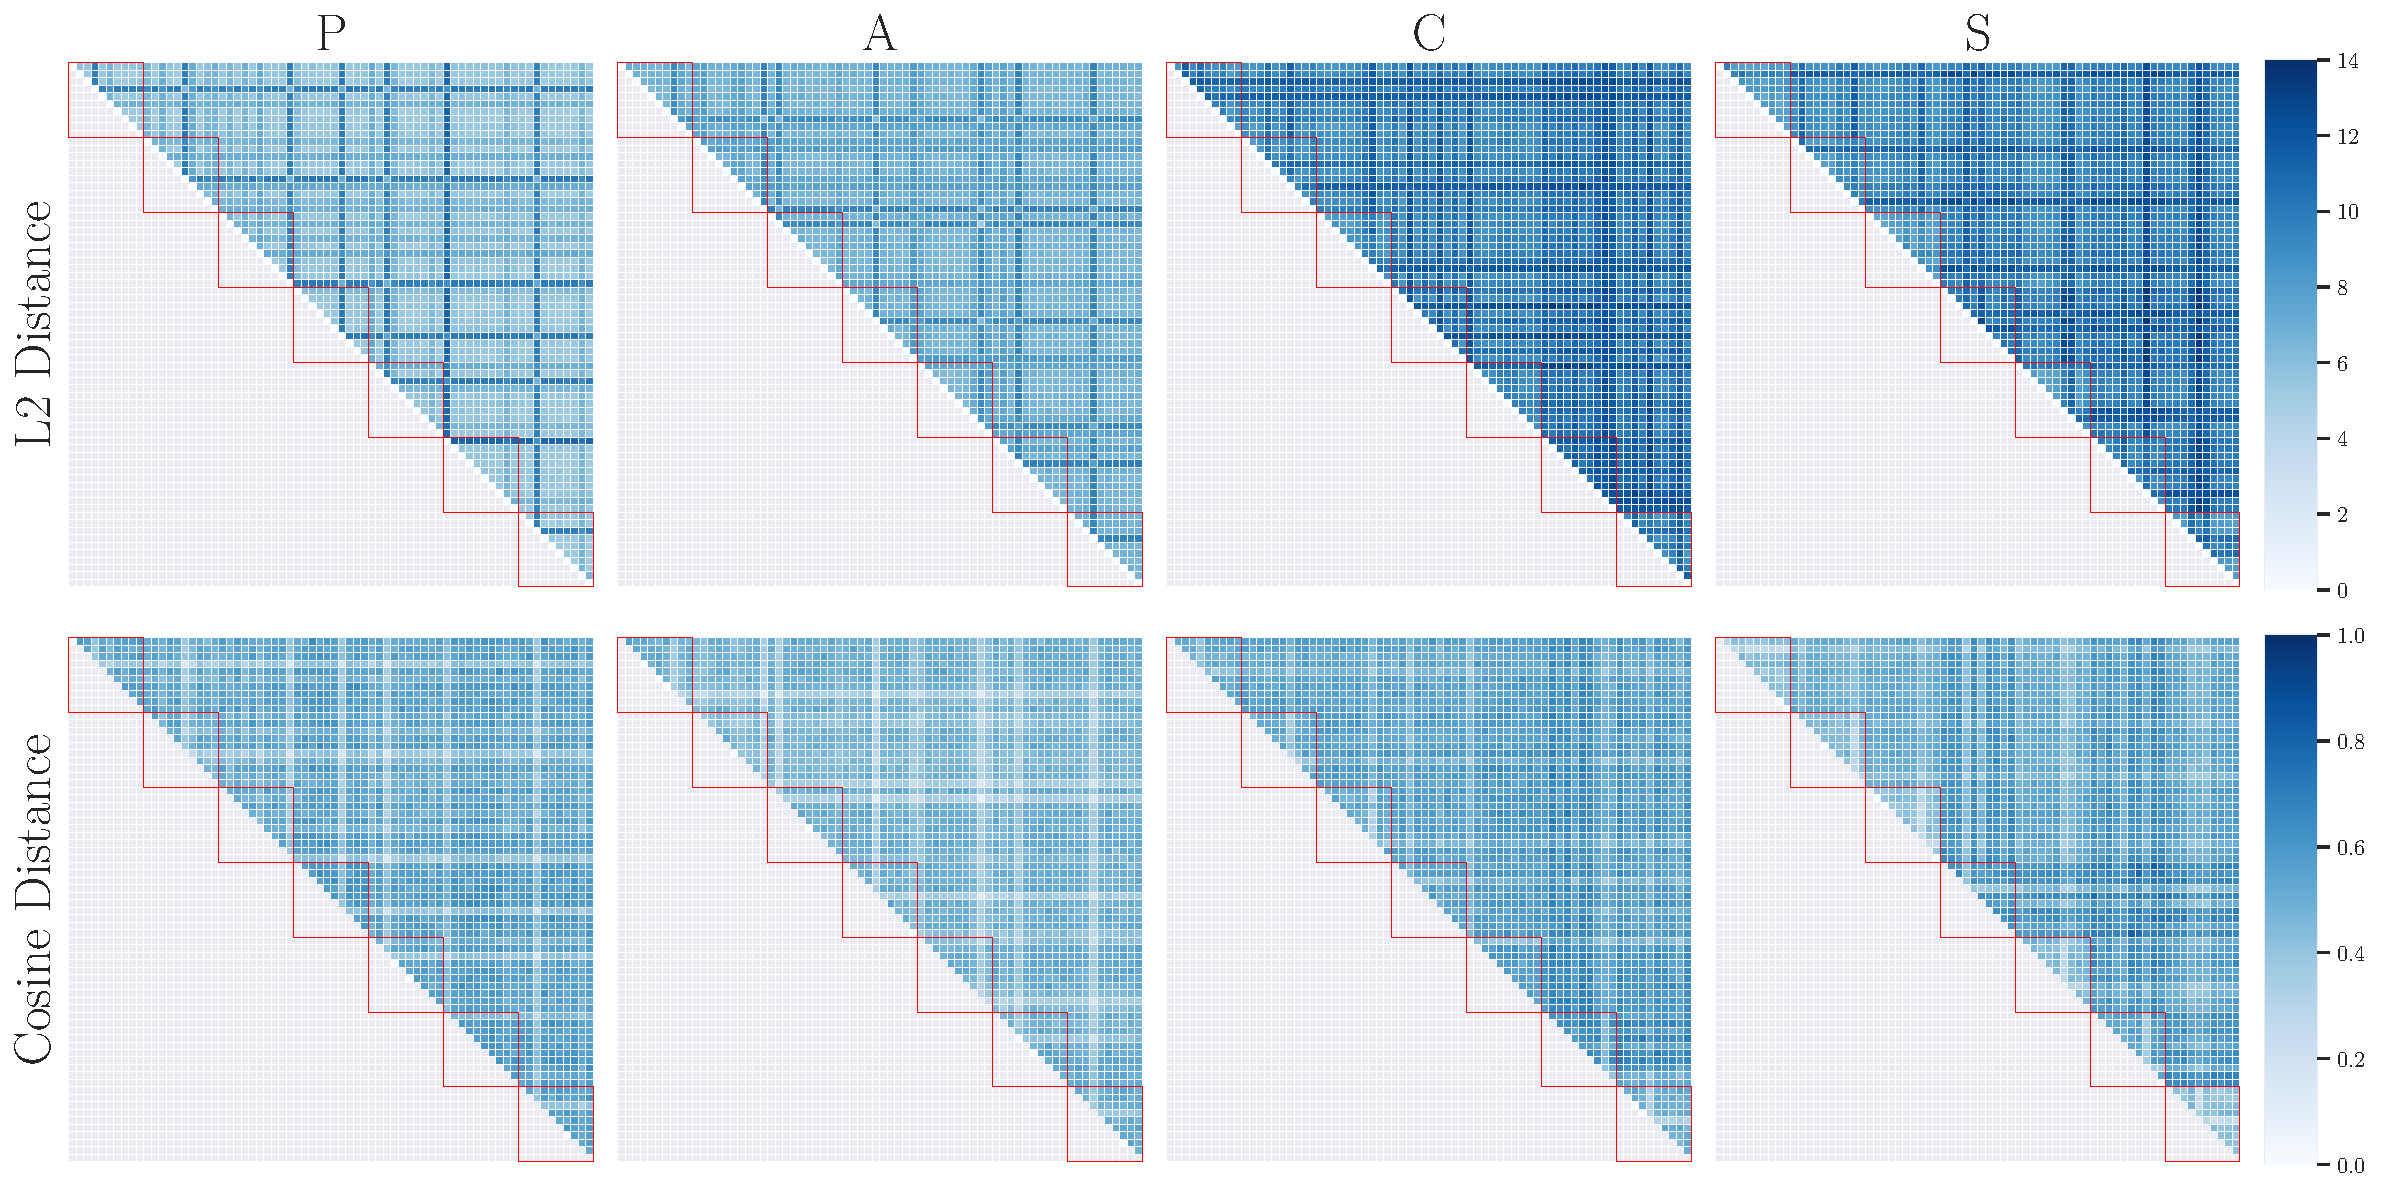
\includegraphics[width=\textwidth]{Figures/Chapter4/2021-01-21-ProDropIncorrectWeight-1.0WithSCdrop_f0.5SAVEResNet18oracle_validation_trial1.pdf}
    \caption[Second data split pairwise self-challenging prototype distances with $w_{c,j} = -1.0$] {Pairwise learned prototype $\ell_2$-distance (top) and cosine-distance $\cdistance$ (bottom) of the best-performing model with negative weight $w_{c,j} = -1.0\; \forall j: \prot \notin \prots_c$ for each testing domain. Red squares denote prototype class correspondence for the $7$ different classes in the PACS dataset. Self-challenging is applied and colormap bounds are adjusted per metric for visualization purposes. Second data split.}
    \label{fig:pw_distance_trial1-sc}
\end{figure}

\paragraph{Influence of the negative weight on the distance metrics}
We also analyze the discrepancies between the distance metrics when comparing $w_{c,j} = -1.0\; \forall j: \prot \notin \prots_c$ and $w_{c,j} = 0.0\; \forall j: \prot \notin \prots_c$ which can be seen in the figures presented in \Cref{sec:additional_distances}. However, from these plots there were no \emph{consistent} trends observable which can be made on how the negative weight influences the training behavior of the prototypes. 

\subsection{Using Support Sets (\dtransformers)}
\label{sec:dtransformers}

Instead of directly learning the set of prototypes $\prots$, we can rely on a support set similar to what is done by \citet{DoerschGZ20} or \citet{SnellSZ17}. Here, the prototypes are based on a support set $\support$ consisting of $n_c$ sample images $\xxi$. This support set exists for each of the classes $c$ as $\supportc = \{\xxic\}_{i=1}^{n_c}$ where $\xxic$ is an image from class $c$. In the classical setting, the set of prototypes for each class $\prots_c$ is then obtained by computing one prototype for each class $\protc$ averaging the average-pooled latent representations of the support set as:
\begin{equation}
    \protc = \frac{1}{|\prots_c|} \sum_{\xxic \in \supportc} \featureex(\xxic)
\end{equation}
Contrary to the previous approach, by averaging all the average-pooled latent representations, there exists only one prototype for each class \ie $|\prots_c| = 1$ and $j=1$ which loses spatial information. Predictions are again made by computing \emph{some} distance function between the prototypes and the latent representation of the image to be classified. \citet{DoerschGZ20} preserve this spatial information of the feature extractor and use the attention weights to guide the averaging across support set images and latent patches in a method that they call \textsc{crossTransformers}. We extend their approach for the domain generalization case here, where we compute attention across multiple training environments. In the following sections this adaptation is referenced as \dtransformers. 

In particular, similar to Transformers \citep{VaswaniSPUJGKP17} and the original idea by \citet{DoerschGZ20}, we use three linear transformations to compute keys, values, and queries. In practice, the key head $\keyh : \mathbb{R}^{K} \mapsto \mathbb{R}^{\dimkey}$, the value head $\valueh : \mathbb{R}^{K} \mapsto \mathbb{R}^{\dimvalue}$, and the query head $\queryh : \mathbb{R}^{K} \mapsto \mathbb{R}^{\dimkey}$  can each be implemented through convolutions with \texttt{kernel\_size = 1}. Prototypes for each domain are computed by passing the support set $\supportc^\env = \{\xxic^\env\}_{i=1}^{n_{\env, c}}$ associated with domain $\env$ and class $c$ through the feature extractor. For each spatial location $m$ in the resulting features (indexed over $H_\mathbf{z} \times W_\mathbf{z}$) of the support set image $i$, we compute dot-product attention scores between keys $\keys = \keyh (\featureex(\xxic^\env))_m$ and the query vectors $\queries = \queryh(\featureex(\xxq^\env))_p$ for a query image $\xxq$ at spatial location $p$ (indexed over $H_\mathbf{z} \times W_\mathbf{z}$). Explicitly, the dot similarity $\attentionw$ between them is computed as:
\begin{equation}
    \attentionw = \keys \cdot \queries.
\end{equation}
Afterwards, we re-scale this dot similarity by using $\scaler=\sqrt{\dimkey}$ and obtain the final attention weights $\attentionwf$ using a \texttt{softmax} operation summing over all spatial locations and images in the support set:
\begin{equation}
    \attentionwf = \frac{\exp(\attentionw / \scaler)}{\sum_{i,m} \exp(\attentionw / \scaler)}.
\end{equation}
Finally, we can use the support-set values $\values = \valueh(\featureex(\xxic^\env))_m$  with the attention weights to compute a prototype vector per spatial location $p$ for each domain and class:
\begin{equation}
    \protipc = \sum_{i,m} \attentionwf \values.
\end{equation}
As a distance, we compute the dot similarity between the prototype and the query image values $\valuesq = \valueh(\featureex(\xxic^\env))_p$ where we sum over the training environments $\env \in \envs$ and the spatial locations $p$ of the query image:
\begin{equation}
    \operatorname{dist}(\xxic, \supportc) = \sum_{\env \in \envs} \frac{1}{H_\mathbf{z} W_\mathbf{z}} \sum_p \protipc \cdot  \valuesq.
\end{equation}
Most notably, we deploy the dot similarity as a distance metric here instead of the squared $\ell^2$-norm used by \citet{DoerschGZ20} since we observe numerical instability for that in our experiments which might be due to the distribution shift in domain generalization. In their work, they reason about using the same value-head $\valueh$ for the queries as used on the support-set images to ensure that the architecture works as a distance \ie if the support set contains the same images as the query, they want the euclidean distance to be $0$ \citep{DoerschGZ20}. Because we observe no performance gains for keeping them separate, we also use the same value head $\valueh$ for both the queries and support set images to reduce additional parameters to a minimum.


